% !TeX root = ../main.tex
% !TeX spellcheck = en_US

\chapter{Case Studies}
\label{ch:casestudiesdeterministic}
Let us now look at some case studies of this framework in practice: How to implement sorting (\autoref{sec:sorting}); how to implement insertion, deletion and searching in a binary search tree (\autoref{sec:trees}); and how to implement a linear-time order statistic computation (\autoref{sec:median}). In each of these cases, we will use the framework developed in the previous chapter to guarantee the respective runtime bounds in the return type of each function.

% !TeX root = ../main.tex
% !TeX spellcheck = en_US

\section{Sorting}
\label{sec:sorting}

As in the introduction, we will consider how to insert an element into an already sorted list. For reference, this is how an insert function would normally look (assuming we had a way to compare elements):

\begin{lstlisting}[caption={Plain insertion},label={lst:insert:plain},emph={insert, if, then, else}]
insert : A -> Vec A l -> Vec A (suc l)
insert e []        = [ e ]
insert e (x :: xs) = if e \leq x
                     then (e :: x :: xs)
                     else (x :: insert e xs)
\end{lstlisting}

And this is how an insertion function looks in our framework:

\noindent\begin{minipage}{\linewidth}
\begin{lstlisting}[caption={Insertion with runtime bound},label={lst:insert:bounded},emph={insert,if,then,else,return}]
insert : A -> Vec A l -> DecTree A (Vec A (suc l)) l
insert e []        = return $ [ e ]
insert e (x :: xs) = if e \leq? x
                     then (return $ e :: x :: xs)
                     else (x ::_ <$> insert e xs)
\end{lstlisting}
\end{minipage}

As we can see, the differences are minor. Let us look at them from top to bottom:

\begin{itemize}
    \item Our original return type is retained, now embedded in the \texttt{DecTree} monad.
    \item The return type also tells us that reducing this computation will take at most $l$ steps.
    \item In lines 2 and 4, at the end of our recursion, we just need to \texttt{return} the result.
    \item In line 5, since the recursive call now returns a \texttt{DecTree}, we lift the vector append function into the monad using the \texttt{<\$>} operator.
\end{itemize}

Let us look at a slightly more complicated example: Merging two sorted vectors by some key function. This is a prerequisite to later implement merge sort.

\begin{lstlisting}[caption={Merging sorted vectors},label={lst:merge},emph={merge,by,DecTree,delay,return,delay',if,then,else}]
merge-by :  (X -> A)
         -> Vec X n -> Vec X m
         -> DecTree A (Vec X (n + m)) (n + m)

merge-by _ []       ys = delay (len ys) $ return ys
merge-by _ (x ∷ xs) [] = delay' (suc n) $ return $ x ∷ xs'
    where
        xs' : Vec X (n + 0)
        xs' = subst (Vec X) (sym $ +-identity\^r n) xs

merge-by f (x ∷ xs) (y ∷ ys) =
        height-\equiv (cong suc \lub-idem-suc-xy) $
        if[ Vec X ] f x \leq? f y
        then (x ∷_ <$> merge-by f xs (y ∷ ys))
        else (y ∷_ <$> merge-by f (x ∷ xs) ys)
            by (cong suc $ sym $ +-suc n' m')
\end{lstlisting}

Again, our return type tells us several things: We return a computation comparing elements of \texttt{A}, the return type of our key function. The result of our computation will be a vector of the combined length of the two input vectors. And our computation will be time-bounded by the length of the returned vector.

In the base case that one of the two vectors is empty, we can immediately return the other vector. However, since this other vector may have a length of more than zero, and our computation is supposed to take as long as the vector is long, we need to insert a delay.

In the second base case, we additionally have the problem that the length of our result vector is \texttt{suc n + 0}. As we have described in the Background chapter (\autoref{sec:tutorial:equality}), it is not immediately obvious to Agda that this is equivalent to a vector of length \texttt{suc n}. Fortunately the Agda standard library provides a function \texttt{+-identity$^r$ : n -> n + 0 $\equiv$ n} which we can use to bring the vector into the right shape.

In the recursive case we have the issue that the two branches' result types are vectors of length \texttt{suc (n + suc m)} and \texttt{suc (suc n + m)} respectively. Again it is not clear to Agda that these two expressions are the same, and again we can manually prove it to Agda using the built-in function \texttt{+-suc : n -> m -> n + suc m $\equiv$ suc (n + m)}.

Finally, the time bound for our execution is \texttt{suc (n + suc m $\sqcup$ suc n + m)}, but we want a time bound of \texttt{suc n + suc m}. We therefore manually provide a proof \texttt{$\sqcup$-idem-suc-xy : n -> m -> suc n + m $\sqcup$ n + suc m $\equiv$ n + suc m}.

With this we can turn towards implementing merge sort, again parameterized by a key function.

\begin{lstlisting}[caption={Mergesort},label={lst:mergesort},emph={DecTree,merge,sort,step,by,recurse,return,delay}]
private
    merge-sort-step :  (X -> A)
                    -> Vec X l
                    -> Acc _<_ l
                    -> DecTree A (Vec X l) (l * \llog l \rceil)

    merge-sort-step _ [] _       = return []
    merge-sort-step _ (x ∷ []) _ = return [ x ]
    merge-sort-step f xs@(_ ∷ _ ∷ _) (Acc.acc more) =
        delay-\leq (log\_2n/2-bound _) $ do
            let (left , right) = split xs

            sorted-left <- merge-sort-step f left
                    (more \lceil l /2\rceil (n>1=>\ndiv2ceil<n _))
            sorted-right <- merge-sort-step f right
                    (more \lfloor l /2\rfloor (n>0=>\ndiv2floor<n _))

            subst (Vec X) (\ndiv2ceil+\ndiv2floor\equivn l) <$>
            merge-by f sorted-left sorted-right


merge-sort : Vec A l -> DecTree A (Vec A l) (l * \llog l \rceil)
merge-sort xs = merge-sort-step id xs $ <-wellFounded l

merge-sort-by :  (X -> A)
              -> Vec X l
              -> DecTree A (Vec X l) (l * \llog l \rceil)
merge-sort-by f xs = merge-sort-step f xs $ <-wellFounded l
\end{lstlisting}

Here we first have to deal with the termination checker. As mentioned in the Background chapter (\autoref{sec:termination-checking}), the termination checker is limited in what it can show as terminating. The splitting of a vector in two exceeds these limits.

In line 4, we are stating that the length of the vector in each call will be strictly decreasing. We prove this in line 14 and 16 with the call to \texttt{more}, the function provided by \texttt{Acc} to produce instances of \texttt{Acc \_<\_ $\lceil$ l /2$\rceil$} and \texttt{Acc \_<\_ $\lfloor$ l /2$\rfloor$} respectively, which allow us to recurse.

We use do-notation to get a nice syntax for writing our implementation. Do-notation de-sugaring in Agda works on a purely syntactic level. On the one hand, this makes it very easy to use do-notation for custom monad-like data structures - no implementation of an actual monad type is needed, just a function named \texttt{\_>\/>=\_} in scope. On the other hand, this purely syntactic substitution can lead to obscure errors if multiple instances of \texttt{\_>\/>=\_} are in scope (for example, for vectors in addition to \texttt{DecTree}) or if the type of \texttt{\_>\/>=\_} is subtly incorrect.

We split the vector in two in line 11 (using a let-binding, since the split function uses no comparisons and thus falls outside our framework). We then sort the two vectors (line 12, 14) and merge the results (line 17). The result of the merge operation is a vector of length $\lceil \frac l 2 \rceil + \lfloor \frac l 2 \rfloor$ and we substitute it for one of length $l$ to match our intended result type in line 16.

The actual run time of our implementation is $\cldiv l * \log_2 \cldiv l + \fldiv l * \log_2 \fldiv l + \cldiv l + \fldiv l$. We bound this from above by $l * \log_2 l$ in line 10 to derive our final bound. The underscore as argument passed to \texttt{log$_2$n/2-bound} tells Agda to attempt and infer the correct argument by unification.

% !TeX root = ../main.tex
% !TeX spellcheck = en_US

\section{Trees}
Trees are an interesting use case for our framework because any operation is going to trivially linear in terms of the height of the tree. Instead, what we'd like to do is frame our run time in terms of the \emph{size} of the tree.

There is two ways we could approach this: We could either bound the height of the tree in terms of the size of the tree while leaving our run-time bounded in terms of the height, or we could track height and size independently and use the size to express our run time.

Since our run time monad already contains a mechanism to express upper instead of strict bounds and since the intuitive way to define a tree data type would have strict bounds, we will use the second approach.

We are going to look at basic binary search trees only. The type is defined as follows:

\begin{lstlisting}[caption={The Tree Type},label={lst:tree:def},emph={Tree,Leaf,Fork}]
data Tree (A : Set a) : bNat -> bNat -> Set a where
    Leaf : Tree A 0 0
    Fork :  {s\_1 s\_2 h\_1 h\_2 : bNat}
         -> Tree A s\_1 h\_1
         -> A
         -> Tree A s\_2 h\_2
         -> Tree A (1 + s\_1 + s\_2) (1 + (h\_1 \lub h\_2))
\end{lstlisting}

It is parameterized by the type of data it contains, and indexed by two natural numbers: The size of the tree (The number of nodes in the tree, excluding leaves for convenience) and the height of the tree (the length of the longest path from the root to a leaf).

We will consider three basic operations of our tree: insertion, removal and test for membership. The membership test is the simplest to implement, so we will start with it.

\begin{lstlisting}[caption={Tree Membership Test},label={lst:tree:contains},emph={Tree,contains,Bool,Leaf,Fork,return,if,then,else}]
contains : Tree A s h -> A -> DecTree A Bool (2 * s)
contains Leaf _ = return false
contains t@(Fork l x r) val =
    height-\equiv (sym $ 2*m\equivm+m $ size t) $
    delay-\leq (s\leqs (comm-\lub\leq+ (size l) (size r))) $
    if val \leq? x
    then height-\equiv (cong suc $ 2*m\equivm+m $ size l) $
         if' x \leq? val
         then delay-\leq z\leqn $ return true
         else contains l val
    else (height-\equiv (2*m\equivm+m $ size r) $ contains r val)
\end{lstlisting}

Here we see one of the shortcomings of the current framework. Since we only have a less-or-equal test as primitive operation, to decide equality we need to spend two comparisons. This not only makes the code structure more complicated, it also makes our bound less neat -- which, due to the recursive calls, forces us to add additional proofs.

A potential solution to this would be to add a primitive that can decide a case of equality, less or greater in one step. Otherwise a wrapper function similar to the alternative if-then-else implementations described in \autoref{ch:detanalysis} in combination with additional support functions for increments-of-two in the depth of a decision tree.

Next, let's look at inserting and removing elements. These operations modify the size of the tree, but may or may not affect the height. How do we express this on the type level? The simple answer would be to return a dependent sum of the new height of the tree and the tree itself. However this way we lose more information than necessary: For insertion, either tree retains its height or it grows by one. For removal, the same is true for the other direction: Either it retains its height or it decreases by one.

The data types to represent this look as follows:

\begin{lstlisting}[caption={Maybe-Increment and Maybe-Decrement},label={lst:tree:inc-type},emph={neutral,decrement}]
data _1?+\langle_\rangle (A : bNat -> Set a) (n : bNat) : Set a where
    +0 : A n       -> A 1?+\langle n \rangle
    +1 : A (suc n) -> A 1?+\langle n \rangle

data _\langle_\rangle-1? (A : bNat -> Set a) : (n : bNat) -> Set a where
    neutral   : A n -> A \langle n \rangle-1?
    decrement : A n -> A \langle suc n \rangle-1?
\end{lstlisting}

We use \texttt{+0} to denote no growth and \texttt{+1} to denote growth by one step. For the decrement type, we instead use full words because names in Agda can not start with a hyphen.

With this in place we can implement our insertion function (some function bodies omitted):

\begin{lstlisting}[caption={Tree Insertion},label={lst:tree:insert},emph={Tree,Fork,Leaf,insert,join,return,if,then,else}]
join-l :  Tree A s\_1 1?+\langle h\_1 \rangle -> A -> Tree A s\_2 h\_2
       -> Tree A (1 + s\_1 + s\_2) 1?+\langle 1 + (h\_1 \lub h\_2) \rangle

join-r :  Tree A s\_1 h\_1 -> A -> Tree A s\_2 1?+\langle h\_2 \rangle
       -> Tree A (1 + s\_1 + s\_2) 1?+\langle 1 + (h\_1 \lub h\_2) \rangle


insert :  Tree A s h
       -> A
       -> DecTree A (Tree A (suc s) 1?+\langle h \rangle) s

insert Leaf x = return $ +1 $ Fork Leaf x Leaf

insert (Fork l x r) val =
    if' val \leq? x
    then (delay-\leq (m\leqm+n _ _) $
          insert l val <&>
          \lambda l' -> join-l l' x r)
    else (delay-\leq (m\leqn+m _ _) $
          insert r val <&>
          \lambda r' -> +-suc-t $ join-r l x r')
  where
    +-suc-t :  Tree A (1 + (s\_1 + suc s\_2)) 1?+\langle h \rangle
            -> Tree A (2 + (s\_1 + s\_2)) 1?+\langle h \rangle
    +-suc-t t = subst (\lambda s -> Tree A s 1?+\langle h \rangle)
                (cong suc $ +-suc _ _) t
\end{lstlisting}

The functions \texttt{join-l} and \texttt{join-r} help us push our maybe-increment operator up a tree level. We will not further concern ourselves with the implementation here.

The actual insertion function is straightforward: Depending on whether the inserted value is smaller or larger than the current root, we insert into the left or right sub-tree and delay the computation so it matches the expected time \texttt{size l + size r} instead of the actual time of \texttt{size l} or \texttt{size r}. The remaining function \texttt{+-suc-t} simply fixes the size of the tree if we insert into the right subtree.

The remaining item for our tree implementation is a removal function, which is not much more complicated than the insertion function. However, first we need to find an algorithm that merges two trees under the assumption that all values in one tree are smaller than all the values in the other tree. We will use this to restore a tree when we remove its root element.

\begin{lstlisting}[caption={Tree Merge},label={lst:tree:merge},emph={Tree,Fork,Leaf,merge,remove,max}]
remove-max : Tree A (suc s) (suc h) -> A × Tree A s 1?+\langle h \rangle

merge :  Tree A s h -> Tree A s' h'
      -> Tree A (s + s') 1?+\langle h \lub h' \rangle
merge Leaf r             = +0 r
merge l@(Fork _ _ _) r with remove-max l
...     | m , +1 l' = +1 $ Fork l' m r
...     | m , +0 l' with ord (height l) (height r)
...         | lt pf = +1 $ tree-\lub-max-< (Fork l' m r) pf
...         | eq pf = +1 $ tree-\lub-max-\equiv (Fork l' m r) pf
...         | gt pf = +0 $ tree-\lub-max-> (Fork l' m r) pf

\end{lstlisting}

The \texttt{remove-max} function does what its name implies: Removing the largest value in a tree and returning it alongside the smaller tree. The merge function uses this to retrieve the largest value from the smaller tree, which is then used as the new root of the reconstructed tree. The remainder of the implementation is just reasoning about the height of the new tree.

This example illustrates another shortcoming of our framework: Merging the two trees may take time \texttt{size l}, but since no comparisons of values inside the tree are necessary for it we can omit this time from the type-level bound.

\begin{lstlisting}[caption={Tree Removal},label={lst:tree:removal},emph={Tree,Fork,Leaf,RemovalTree,return,if,then,else,neutral,decrement,remove}]
RemovalTree : Set a -> bNat -> bNat -> Set a
RemovalTree A s h = _\langle_\rangle-1? (\lambda s' -> Tree A s' \langle h \rangle-1?) s

remove :  Tree A s h -> A
       -> DecTree A (RemovalTree A s h) (2 * s)
remove Leaf val = return $ neutral $ neutral Leaf
remove (Fork l x r) val =
    height-\equiv (sym $ 2*m\equivm+m s) $
    delay-\leq (s\leqs $ comm-\lub\leq+ (size l) (size r)) $
    if val \leq? x
    then height-\equiv (cong suc $ 2*m\equivm+m $ size l) $
         if' x \leq? val -- x \leq val + val \leq x => x \equiv val
         then delay-\leq (z\leqn) $
              return $ remove-merge $ merge l r
         else (remove l val <&> \lambda l' -> remove-join-l l' x r)
    else (height-\equiv (2*m\equivm+m $ size r) $
         remove r val <&> \lambda r' -> remove-join-r l x r')
where
    h-1 : bNat
    h-1 = height l \lub height r
    remove-merge :  Tree A (size l + size r)
                        1?+\langle height l \lub height r \rangle
                 -> RemovalTree A s h
    remove-merge (+0 t) = decrement $ decrement t
    remove-merge (+1 t) = decrement $ neutral t
    remove-join-l :  RemovalTree A (size l) (height l)
                  -> A
                  -> Tree A (size r) (height r)
                  -> RemovalTree A s h
    remove-join-r :  Tree A (size l) (height l)
                  -> A
                  -> RemovalTree A (size r) (height r)
                  -> RemovalTree A s h
\end{lstlisting}

A removal can, but does not need to, decrease both the size and the height of the tree. Since the type for this becomes cumbersome to write, we introduce the type alias \texttt{RemovalTree}.

The body of \texttt{remove} is similar to \texttt{contains}: Again we check both $val \leq x$ and $x \leq val$ to determine equality. This increases our running time to $2s$ which incurs additional proof burden.

The two distinct cases are finding the element in the tree or removing it from one of the sub trees. In the first case, we simply merge the two sub trees with the algorithm described earlier and then convert the result into a \texttt{RemovalTree}. In the second case we have the functions \texttt{remove-join-l} and \texttt{remove-join-r}, which take the result of the recursive call as well as the current root and the other sub tree and massage this into a \texttt{RemovalTree}..
% !TeX root = ../main.tex
% !TeX spellcheck = en_US

\section{Median and Order Statistics}
\label{sec:median}
Our final case study is concerned with computing order statistics. The $k$-th order statistic is the $k$-th smallest value in a set. The median is a special case of an order statistic with $k = \frac n 2$. The obvious approach to calculating order statistics is to first sort the set and then select the value at index $k$. With a sorting algorithm, this can be done in time $\mathcal O(n \log n)$. However we can do better: The quickselect algorithm of Hoare \cite{hoare:1961:quickselect} calculates order statistics in linear time. The algorithm works by quickly identifying the top and bottom 30\% of values so in each iteration we can eliminate a significant chunk of the data set.

Often we are not only interested in what the $k$th order statistics is, but also where to find it in the original data set, and which values are smaller or larger than it. We calculate this information anyway, so we return it alongside the actual value.

\noindent\begin{minipage}{\linewidth}
\begin{lstlisting}[caption={The Indexed type},label={lst:median:indexed},emph={Indexed,index}]
record Indexed (A : Set a) (l : bNat) : Set a where
    constructor index
    field
        idx : Fin l
        value : A
\end{lstlisting}
\end{minipage}

To store the index of a value, we use Agda's finite number type: the type \texttt{Fin l} contains all natural numbers smaller than $l$. The element \texttt{zero} is part of every \texttt{Fin l}  for $l > 0$ and any other element of some \texttt{Fin (suc l)} is constructed as the successor of a number in \texttt{Fin l}.

\begin{lstlisting}[caption={The Split type},label={lst:median:split},emph={Split,Indexed}]
record Split (A : Set a) (l : bNat) (b\_1 b\_2 : bNat -> Set) : Set a
    where
    field
        median : Indexed A l
        {l\_1 l\_2 l\_3} : bNat
        smaller : Vec (Indexed A l) l\_1
        larger : Vec (Indexed A l) l\_2
        unknown : Vec (Indexed A l) l\_3
        length-≡ : suc (l\_1 + l\_2 + l\_3) ≡ l
        bound-smaller : b\_1 l\_1
        bound-larger : b\_2 l\_2
\end{lstlisting}

The \texttt{Split} type, which will form the return type of our median and quickselect functions, is parameterized by four values: The type from which we will draw our values, the size of the set analyzed and two constraint types, indexed by the naturals. The record stores the median value, as well as the remainder of the analyzed set split into a smaller and a larger section and one of which we do not have ordering information.

We guarantee that a \texttt{Split} instance contains the entirety of the originally analyzed set by proxy: by showing that the length of the three subsets plus the median element itself sum up to the original length.

Finally, we have two bounds, for the size of the smaller and the larger subset. This allows us to express the guarantee of the intermediate elimination described above:

\noindent\begin{minipage}{\linewidth}
\begin{lstlisting}[caption={Intermediate function (sketch)}]
intermediate :  Vec A l
             -> Split A l (_\geq 3 * (l / 10)) (_\geq 3 * (l / 10))
\end{lstlisting}
\end{minipage}

As well as that of our final functions such as the median:

\noindent\begin{minipage}{\linewidth}
\begin{lstlisting}[caption={Median function (sketch)}]
median :  Vec A l
       -> Split A l (_\equiv \lfloor l /2\rfloor) (_\equiv \lceil l /2\rceil - 1)
\end{lstlisting}
\end{minipage}


Our intermediate step works as follows: We group our data into sets of five. We can order the elements of each of these sets with respect to their median in constant time (\autoref{fig:median-of-5}).

\begin{figure}[h]
\begin{center}
        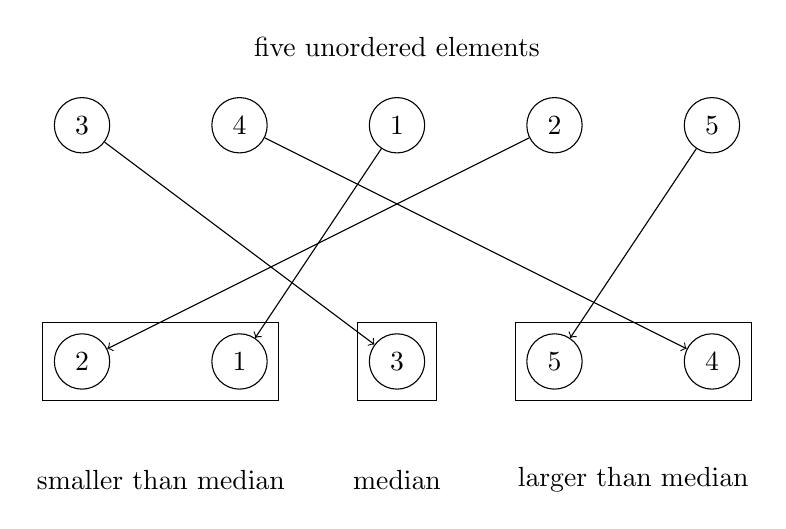
\begin{tikzpicture}

\node [shape=circle, draw=black, minimum size=2em] (v1) at (-3,1.5) {3};
\node [shape=circle, draw=black, minimum size=2em] (v3) at (-1,1.5) {4};
\node [shape=circle, draw=black, minimum size=2em] (v5) at (1,1.5) {1};
\node [shape=circle, draw=black, minimum size=2em] (v7) at (3,1.5) {2};
\node [shape=circle, draw=black, minimum size=2em] (v9) at (5,1.5) {5};
\node [shape=circle, draw=black, minimum size=2em] (v8) at (-3,-1.5) {2};
\node [shape=circle, draw=black, minimum size=2em] (v6) at (-1,-1.5) {1};
\node [shape=circle, draw=black, minimum size=2em] (v2) at (1,-1.5) {3};
\node [shape=circle, draw=black, minimum size=2em] (v10) at (3,-1.5) {5};
\node [shape=circle, draw=black, minimum size=2em] (v4) at (5,-1.5) {4};
\draw [->] (v1) edge (v2);
\draw [->] (v3) edge (v4);
\draw [->] (v5) edge (v6);
\draw [->] (v7) edge (v8);
\draw [->] (v9) edge (v10);
\node at (1,-3) {median};
\node at (-2,-3) {smaller than median};
\node at (4,-3) {larger than median};
\draw [->] (-3.5,-1) rectangle (-0.5,-2);
\draw [->] (2.5,-1) rectangle (5.5,-2);
\draw [->] (0.5,-1) rectangle (1.5,-2);
\node at (1,2.5) {five unordered elements};
\end{tikzpicture}
\end{center}
\caption{Median of 5}
\label{fig:median-of-5}
\end{figure}

\begin{lstlisting}[caption={Median of 5},label={lst:median:medofmeds},emph={M,median,by,medians,of}]
M5 : Set a -> bNat -> Set a
M5 A l = Indexed A l × Indexed A l -- the two smaller elements
       × Indexed A l               -- the median
       × Indexed A l × Indexed A l -- the two larger elements

median5-by :  (X -> A)
           -> X -> X -> X -> X -> X
           -> DecTree A (M5 X 5) 7


data Medians-Of-5 (A : Set a) (l : bNat) : Set a where
    medians :  Vec (M5 A l) \lfloor l /5\rfloor
            -> Vec (Indexed A l) (l % 5)
            -> Medians-Of-5 A l

_:::_ : M5 A 5 -> Medians-Of-5 A l -> Medians-Of-5 A (5 + l)


medians-of-5-by :  (X -> A) -> Vec X l
                -> DecTree A (Medians-Of-5 X l) (2 * l)
medians-of-5-by _ [] =
        return $ medians [] []
medians-of-5-by _ (a :: []) =
        delay 2 $
        return $ medians [] [ index f0 a ]
medians-of-5-by _ (a :: b :: []) =
        delay 4 $
        return $ medians [] $  (index f0 a)
                            :: [ index f1 b ]
medians-of-5-by _ (a :: b :: c :: []) =
        delay 6 $
        return $ medians [] $  (index f0 a)
                            :: (index f1 b)
                            :: [ index f2 c ]
medians-of-5-by _ (a :: b :: c :: d :: []) =
        delay 8 $
        return $ medians [] $  (index f0 a)
                            :: (index f1 b)
                            :: (index f2 c)
                            :: [ index f3 d ]
medians-of-5-by f (a :: b :: c :: d :: e :: xs) =
        let n = len xs in
        height-\equiv (sym $ *-distrib\^l-+ 2 5 n) $
        height-\equiv (cong (10 +_) $ +-identity\^r (2 * n)) $ do
        m5 <- delay 3 $ median5-by f a b c d e
        ms <- medians-of-5-by f xs
        return $ m5 ::: ms

\end{lstlisting}

The type \texttt{M5} (lines 1-4) over some type \texttt{A} is a 5-tuple of indexed elements of \texttt{A}, which represents the median of these five values alongside the smaller and larger elements.

The type \texttt{Medians-Of-5} (lines 11-14) represents the results of mapping this selection of the median of five elements over a full list. It contains a vector of the \texttt{M5} tuples that result from grouping the original data set into sets of five and selecting their respective median (line 12). Since the input data set's size may not be evenly divisible by five, we also store the remaining elements (line 13). The function \texttt{\_:::\_} prepends a median of five to the full result set, making sure to adjust the indices as required.

Finally, we implement the actual medians-of-5 function (lines 19ff.). We ignore the final remainder of the list if it is not divisible by 5 (see the cases in lines 23, 26, 30 and 35), and map our five-element median function over the rest (lines 45 and 46). Each step takes us slightly less than 10 units of time per five elements, and we bound this from above as two times the total size of the set.

Having done that, we can order these sets-of-5 \emph{themselves} by comparing their median values. By transitivity we know that in each set that is smaller than the median set, the leftmost three items are smaller than the median of the median values. This also holds symmetrically for the larger sets (see \autoref{fig:median-of-medians}).

\begin{figure}
\begin{center}
    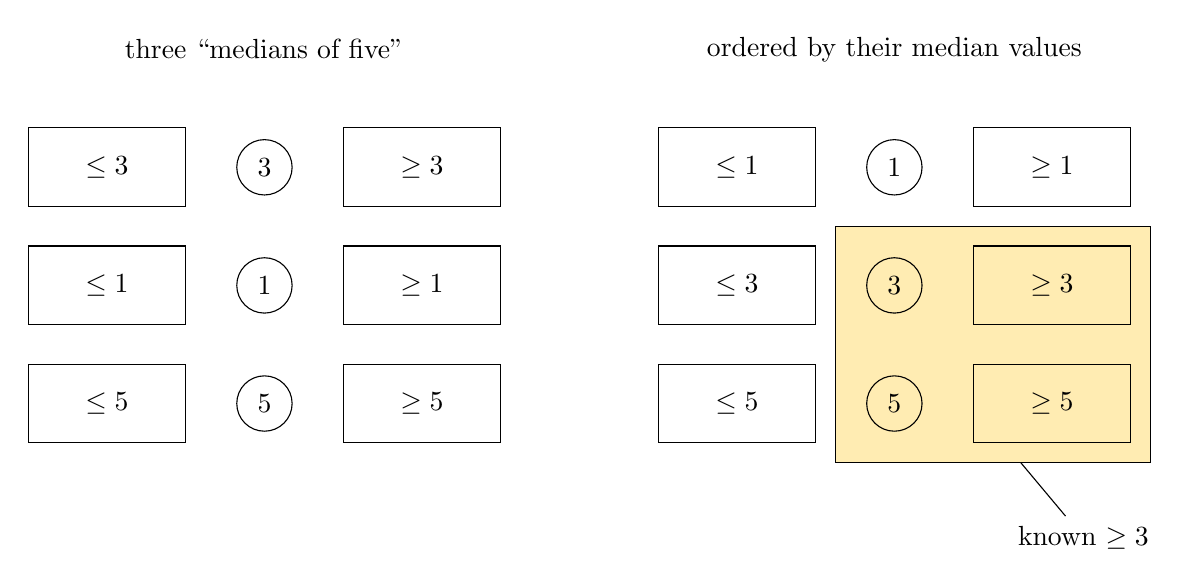
\begin{tikzpicture}
\definecolor{amber}{rgb}{1.0, 0.75, 0.0}

\draw [fill=amber, fill opacity=0.3] (7.25,3.75) rectangle (11.25,0.75);

\draw  (-3,5) rectangle (-1,4);
\node [shape=circle, draw=black, minimum size=2em] at (0,4.5) {3};
\draw  (1,5) rectangle (3,4);
\draw  (-3,3.5) rectangle (-1,2.5);
\draw  (1,3.5) rectangle (3,2.5);
\draw  (-3,2) rectangle (-1,1);
\draw  (1,2) rectangle (3,1);
\node [shape=circle, draw=black, minimum size=2em] at (0,3) {1};
\node [shape=circle, draw=black, minimum size=2em] at (0,1.5) {5};
\node at (0,6) {three ``medians of five"};
\node at (-2,4.5) {$\leq 3$};
\node at (2,4.5) {$\geq 3$};
\node at (-2,3) {$\leq 1$};
\node at (2,3) {$\geq 1$};
\node at (-2,1.5) {$\leq 5$};
\node at (2,1.5) {$\geq 5$};
\node at (4,3) {$\implies$};
\draw  (5,5) rectangle (7,4);
\draw  (9,5) rectangle (11,4);
\draw  (5,3.5) rectangle (7,2.5);
\draw  (9,3.5) rectangle (11,2.5);
\draw  (5,2) rectangle (7,1);
\draw  (9,2) rectangle (11,1);
\node [shape=circle, draw=black, minimum size=2em] at (8,4.5) {1};
\node [shape=circle, draw=black, minimum size=2em] at (8,3) {3};
\node [shape=circle, draw=black, minimum size=2em] at (8,1.5) {5};
\node at (8,6) {ordered by their median values};
\node at (6,4.5) {$\leq 1$};
\node at (10,4.5) {$\geq 1$};
\node at (6,3) {$\leq 3$};
\node at (10,3) {$\geq 3$};
\node at (6,1.5) {$\leq 5$};
\node at (10,1.5) {$\geq 5$};
\node (v1) at (10.4,-0.2) {known $\geq 3$};
\node (v2) at (9.5,0.875) {};
\draw  (v1) edge (v2);
\end{tikzpicture}
\end{center}
\caption{Median of medians}
\label{fig:median-of-medians}
\end{figure}

How do we select the median-of-medians? We fall back to the function we wanted to implement originally -- the median selection itself, now on the reduced data set of $\lfloor \frac n 5 \rfloor$.

\noindent\begin{minipage}{\linewidth}
\begin{lstlisting}[caption={Quasi-median and order statistic signatures},label={lst:median:quasimedian},emph={Quasi,Median,quasi,median,by,ordselect,Ordselect}]
Quasi-Median : Set a -> bNat -> Set a
Quasi-Median A l = Split A l
                   (\lambda x -> suc x \geq 3 * (l / 10))
                   (\lambda x -> suc x \geq 3 * (l / 10))

quasi-median-by :  let l = suc l-1 in
                   Acc _<_ l
                -> (X -> A)
                -> Vec X l
                -> DecTree A (Quasi-Median X l) (9 * l)

Ordselect : Set a -> (l : bNat) -> (i : Fin l) -> Set a
Ordselect A l i = Split A l
                  (_\equiv Data.Fin.tobNat i)
                  (_\equiv l Data.Fin.bNat-bNat (Data.Fin.raise 1 i))

ordselect-by :  let l = suc l-1 in
                Acc _<_ l
             -> (X -> A)
             -> (i : Fin l)
             -> (xs : Vec X l)
             -> DecTree A (Ordselect X l i) (35 * l)
\end{lstlisting}
\end{minipage}

Since our functions are mutually recursive, we have to pass an accessibility proof again. As with our sorting algorithms, we will show termination by way of the length of the vector.

Our elimination function will return a quasi-median (lines 1-4): A split that guarantees that 30\% (strictly speaking: $3 \cdot \lfloor \frac l {10}\rfloor$) of elements are smaller and greater than the selected median value. We furthermore guarantee that this is achievable in linear time with constant factor 9 (line 10).

In a similar vein, our ordselect (\emph{order statistic selection}) algorithm will return a split that guarantees that exactly $i$ elements are smaller than the $i$th order statistic and the remaining $l - i - 1$ elements are larger (lines 12-15). This too, is achievable in linear time, with constant factor 35.

\newpage
\begin{lstlisting}[caption={Quasi-median},label={lst:median:quasimedian}]
{- Cases for vectors of less than 5 elements omitted -}
quasi-median-by (Acc.acc more) f
                xs@(_ ∷ _ ∷ _ ∷ _ ∷ _ ∷ xss) =
    let l = suc l-1 in
    height-\equiv (sym $ *-distrib\^r-+ l 2 7) $
    height-\equiv (+-identity\^r (2 * l + 7 * l)) $
    height-\equiv (sym $ +-assoc (2 * l) (7 * l) 0 ) $
    do
        medians ms overflow <- medians-of-5-by f xs
        let ix = ix-half ms
        med-of-meds' <- delay-\leq (a*5*\lfloorn/5\rfloor\leqa*n 7 l) $
                        ordselect-by
                            (more \lfloor l /5\rfloor $ \lfloorl/5\rfloor<l _)
                            (f \circ m5-extract-value) ix ms
        let med-of-meds = simplify-med-split med-of-meds'
        return $ record
            { median = m5-extract-indexed $
                       Indexed.value $
                       Split.median med-of-meds
            ; smaller = small med-of-meds
            ; larger = large med-of-meds
            ; unknown = unk med-of-meds ++ overflow
            ; length-≡ = quasi-median-length-\equiv $ len xss
            ; bound-smaller = \leq-step $ \leq-step $ \leq-step \leq-refl
            ; bound-larger = a+a*n/10\geqa*\lceiln+5\rceil/10 3 (len xss)
            }
  where
    m5-extract-value    :  M5 A l -> A

    ix-half : Vec A (suc l-1) -> Fin (suc l-1)
    ix-half _ = frombNat< {m = \lfloor suc l-1 /2\rfloor} (n>0=>\lfloorn/2\rfloor<n _)

    simplify-med-split : let l = 5 + l-5 in
                   Ordselect (M5 A l) \lfloor l /5\rfloor (ix-half v)
                -> Split (M5 A l) \lfloor l /5\rfloor
                         (_\equiv \lfloor \lfloor l /5\rfloor /2\rfloor)
                         (_\equiv \lfloor \lfloor l-5 /5\rfloor /2\rfloor)

    small :  let l = 5 + l-5 in
             Split (M5 A l) \lfloor l /5\rfloor
                   (_\equiv \lfloor \lfloor l /5\rfloor /2\rfloor)
                   (_\equiv \lfloor \lfloor l-5 /5\rfloor /2\rfloor)
          -> Vec (Indexed A l) (2 + 3 * (l / 10))

    large :  let l = 5 + l-5 in
             Split (M5 A l) \lfloor l /5\rfloor
                   (_\equiv \lfloor \lfloor l /5\rfloor /2\rfloor)
                   (_\equiv \lfloor \lfloor l-5 /5\rfloor /2\rfloor)
          -> Vec (Indexed A l) (2 + 3 * (l-5 / 10))

    unk :  let l = 5 + l-5 in
           Split (M5 A l) \lfloor l /5\rfloor
                 (_\equiv \lfloor \lfloor l /5\rfloor /2\rfloor)
                 (_\equiv \lfloor \lfloor l-5 /5\rfloor /2\rfloor)
        -> Vec (Indexed A l) (2 * (l / 10) + 2 * (l-5 / 10))
\end{lstlisting}

We finally get to (one half of) the meat of our order statistic algorithm. For our quasi-median function, we first group our vector into ordered sets of five (line 9). We then select the \emph{actual} median of these sets, specifying that we want to order them by their middle value (line 11-14).

Selecting this median takes time $35 \cdot \lfloor \frac l 5 \rfloor$. We rewrite this in as a multiple of $l$ by showing that $35 \cdot \lfloor \frac l 5 \rfloor \leq 7 l$ (which, as most mathematical proofs in Agda is surprisingly non-trivial) in line 11.

Since the bounds for the size of the smaller and the larger section of quickselect's split are expressed in terms of the \texttt{Fin} number type, we reframe this in the \texttt{Nat} type by showing that the bounds are equivalent to $\lfloor \lfloor \frac l 5 \rfloor / 2 \rfloor$ and $\lfloor \lfloor \frac {l - 5} 5 \rfloor / 2 \rfloor$, respectively (line 15, using the function defined in line 33-37).

Finally, we extract the part that we are \emph{sure} is smaller than the selected median-of-medians (the ``top left" section in \autoref{fig:median-of-medians}) and similarly for the larger section (lines 20 and 21, respectively). Everything else, including the leftover elements that we could not group into sets of five, end up in the unknown block.

What remains is largely the mathematical proof burden to show that all of our bounds hold.

\begin{lstlisting}[caption={Quickselect (signature)},label={lst:median:quickselect},emph={ordselect,by}]
ordselect-by :  let l = suc l-1 in
                Acc _<_ l
             -> (X -> A)
             -> (i : Fin l)
             -> (xs : Vec X l)
             -> DecTree A (Ordselect X l i) (35 * l)

ordselect-by wf-acc f i xs with \leq-total (suc l-1) 8000
\end{lstlisting}

Finally, we come to an algorithmic sleight of hand: We can only prove that our quickselect bound holds when the length of the input is larger than 8000 (\autoref{lst:median:quickselect}, line 8): Whether we eliminate the larger or the smaller section of our quasi-median split, we can show that the length of the remainder (smaller and unknown or larger and unknown) is less than $7 \cdot \lfloor\frac l {10}\rfloor + 9$. To prove our desired bound of $35l$ for the whole of the algorithm, we need to show that recursing on this remainder (nominally $35\cdot(7 \cdot \lfloor\frac l {10} \rfloor + 9)$) is less than $25l$. However, the constant $+~9$ is getting in our way. We can rewrite the length of the vector as $70 \cdot \lfloor\frac l {100}\rfloor + 79$, which, under the assumption that $l > 800$, is less than $71 \cdot \lfloor\frac l {100}\rfloor$. With the constant so eliminated, we can eventually prove that the recursive call completes in time $25l$. The full proof is listed below.

However, for $l < 8000$, $\lceil \log_2 l \rceil$ is always below $13$ -- well within our bound! We therefore fall back to the sorting approach for this case, using our linear approach only where we can show it is within our (generous) bound.

\begin{lstlisting}[caption={Quickselect ($l \leq 8000$)},label={lst:median:quickselect:small},emph={ordselect,by,split,sorted,merge,sort}]
ordselect-by wf-acc f i xs with \leq-total (suc l-1) 8000
... | inj\_1 l\leq8000 = delay-\leq nlogn\leq35n $
                    split-sorted i <$> sorted
  where
    nlogn\leq35n : l * \lceillog\_2 l \rceil \leq 35 * l
    nlogn\leq35n = begin
        l * \lceillog\_2 l \rceil  \leq\langle *-mono\^r-\leq l $
                          n\leq8000=>\lceillog\_2n\rceil\leq35 l\leq8000 \rangle
        l * 35         \equiv\langle *-comm l 35 \rangle
        35 * l        \qed
    sorted = merge-sort-by (f \circ Indexed.value) $
             zipWith index (allFin l) xs
\end{lstlisting}

We index all the elements in the list, sort it and then split it at the specified location. Then we simply have to show that sorting the list is indeed faster than $35l$. For this proof (\texttt{nlogn$\leq$35n}, line 5-10) we introduce new notation: Equational reasoning. Equational reasoning relates two values (\texttt{l * $\lceil$log$_2$ l $\rceil$} in line 7 with \texttt{35 * l} in line 10) via a series of intermediate step. In our case, the relation will be $\leq$, specified by opening the module \texttt{Nat.Properties.$\leq$-Reasoning}.

The intermediate steps are related to each other by the functions \texttt{\_$\leq$$\langle$\_$\rangle$\_} and \texttt{\_$\equiv$$\langle$\_$\rangle$\_} which are effectively a way to write transitivity proofs in-line. The two functions are right-associative, thus we start analyzing this block of code from the end: the symbol $\qed$ is actually the function \texttt{\_$\qed$ : (x : $\mathbb N$) -> x $\leq$ x}, i.e. it just takes a value (in this case \texttt{35 * l}) and shows that it is related to itself. The function \texttt{\_$\leq$$\langle$\_$\rangle$\_} takes a value $x$ on the one side, a proof of $y \leq z$ on the other side and in between the angular brackets a proof that $x \leq y$ and yield a proof that $x \leq z$. The function \texttt{\_$\equiv$$\langle$\_$\rangle$\_} does the same, but in the brackets takes a proof of $x \equiv y$ instead. By chaining these methods, we can step by step construct a more complicated proof of one value being less or equal to another.


\begin{lstlisting}[caption={Quickselect ($l > 8000$)},label={lst:median:quickselect:large},emph={ordselect,by}]
ordselect-by wf-acc f i xs with \leq-total (suc l-1) 8000
... | inj\_2 l>8000 =
    let ibNat = tobNat i in
    height-\equiv (sym $ *-distrib\^r-+ l 9 26) $ do
        split <- quasi-median-by wf-acc f xs
        let l\_1 = Split.l\_1 split
        let l\_2 = Split.l\_2 split
        let l\_3 = Split.l\_3 split
        let median = Split.median split
        let unknown = Split.unknown split
        let l\_3\leql = \leq-trans
                     (m\leqn+m l\_3 (1 + l\_1 + l\_2))
                     (\leq-reflexive $ Split.length-\equiv split)
        unk-smaller , unk-larger by us+ul\equivl₃ <-
            delay-\leq l\_3\leql $
            split-pivot-by (f \circ Indexed.value) median unknown
        let smaller = Split.smaller split ++ unk-smaller
        let larger  = Split.larger  split ++ unk-larger
        let us\leql\_3 = \leq-trans
                      (m\leqm+n (len unk-smaller)
                             (len unk-larger))
                      (\leq-reflexive us+ul\equivl\_3)
        let ul\leql\_3 = \leq-trans
                      (m\leqn+m (len unk-larger)
                             (len unk-smaller))
                      (\leq-reflexive us+ul\equivl\_3)

        case ord ibNat (len smaller) of \lambda where
            (lt pf) -> delay-\leq (smallerRuntimeBound
                                    split
                                    (len unk-smaller)
                                    us\leql\_3) $
                       ordselect-lt
                           wf-acc f i
                           (Split.median split)
                           smaller larger
                           us+ul\equivl\_3
                           (Split.length-\equiv split)
                           pf
            (eq pf) -> delay-\leq z\leqn $ return $
                       ordselect-eq
                           i
                           (Split.median split)
                           smaller larger
                           us+ul\equivl\_3
                           (Split.length-\equiv split)
                           pf
            (gt pf) -> delay-\leq (largerRuntimeBound
                                    split
                                    (len unk-larger)
                                    ul\leql\_3) $
                       ordselect-gt
                           wf-acc f i
                           (Split.median split)
                           smaller larger
                           us+ul\equivl\_3
                           (Split.length-\equiv split)
                           pf
\end{lstlisting}

We first select the quasi median of the provided data in time $9l$ (line 5). We then further split the unknown data set into a larger and a smaller part with respect to this quasi median in time $l$ (line 14-16). Finally, we see how the length of the smaller data set compares to the index we are looking for (line 28): If the index is smaller, we just select with the same index from the smaller data set (case starting at line 29). If the index is equal, we simply return the selected quasi median (case starting at line 40). And if the index is larger, we subtract the size of the smaller data set from the index and use this to select from the larger data set (case starting in line 48).

As for the runtime, we show that selecting the median from the smaller or larger data set, which runs in time $35 \cdot \abs{\mathrm{\texttt{smaller}}}$ or $35 \cdot \abs{\mathrm{\texttt{larger}}}$ respectively, is faster than $25l$. Let us inspect this proof for the smaller case. The larger case follows by symmetry.

From the selection of the quasi-median, we know that

\[1 + \abs{\mathrm{\texttt{smaller}}_q} + \abs{\mathrm{\texttt{larger}}_q} + \abs{\mathrm{\texttt{unknown}}} = l\]

\vskip 1em
and

\[1 + \abs{\mathrm{\texttt{larger}}_q} \geq 3 \cdot \lfloor \frac l {10} \rfloor\]

where $\mathrm{\texttt{smaller}}_q$ and $\mathrm{\texttt{larger}}_q$ represent the Split sections returned by the quasi-median, in contrast with $\mathrm{\texttt{smaller}}_u$, which is the smaller part of the \texttt{unknown} section and $\mathrm{\texttt{smaller}}$, which is the concatenation of the former two.

We split the unknown set into a smaller and a larger set and add it to the smaller and larger set of the quasi median and thus have

\[\abs{\mathrm{\texttt{smaller}}} = \abs{\mathrm{\texttt{smaller}}_q} + \abs{\mathrm{\texttt{smaller}}_u}\]
\[\abs{\mathrm{\texttt{larger}}} = \abs{\mathrm{\texttt{larger}}_q} + \abs{\mathrm{\texttt{larger}}_u}\]
\[1 + \abs{\mathrm{\texttt{smaller}}} + \abs{\mathrm{\texttt{larger}}} = l\]

\vskip 1em
and by transitivity of $\leq$

\[1 + \abs{\mathrm{\texttt{larger}}} \geq 3 \cdot \lfloor \frac l {10} \rfloor.\]

\vskip 1em
Now we can show that

\begin{alignat*}{1}
    &\quad \abs{\mathrm{\texttt{smaller}}} \\
    =&\quad l - (1 + \abs{\mathrm{\texttt{larger}}}) \\
    \leq&\quad l - 3 \cdot \lfloor \frac l {10} \rfloor \\
    =&\quad l \bmod 10 + 10 \cdot \lfloor \frac l {10} \rfloor - 3 \cdot \lfloor \frac l {10} \rfloor \\
    =&\quad l \bmod 10 + 7 \cdot \lfloor \frac l {10} \rfloor \\
    \leq&\quad 7 \cdot \lfloor \frac l {10} \rfloor + 9.
\end{alignat*}

Under the assumption that $l \geq 8000$, we can further generalize this to

\begin{alignat*}{1}
    &\quad 7 \cdot \lfloor \frac l {10} \rfloor + 9 \\
    =&\quad 7 \cdot \lfloor \frac {10l} {100} \rfloor + 9 \\
    \leq&\quad 70 \cdot \lfloor \frac {l} {100} \rfloor + 79 \\
    \leq&\quad 70 \cdot \lfloor \frac {l} {100} \rfloor + \lfloor \frac {8000} {100} \rfloor \\
    \leq&\quad 70 \cdot \lfloor \frac {l} {100} \rfloor + \lfloor \frac {l} {100} \rfloor \\
    =&\quad 71 \cdot \lfloor \frac {l} {100} \rfloor.
\end{alignat*}

And thus selecting an order statistic from the smaller set takes time

\begin{alignat*}{1}
    &\quad 35 \cdot 71 \cdot \lfloor \frac {l} {100} \rfloor \\
    \leq&\quad 2500 \cdot \lfloor \frac {l} {100} \rfloor \\
    \leq&\quad 25 l.
\end{alignat*}

Knowing this, we can conclude that selecting the quasi median (time $9l$), splitting the unknown section (time $l$) and recursing on the appropriate smaller section (time $25l$) together takes total time $35l$, which is exactly the bound we wanted to show.